\documentclass[12pt, twoside]{article}
\usepackage[letterpaper, margin=1in, headsep=0.5in]{geometry}
\usepackage[english]{babel}
\usepackage[utf8]{inputenc}
\usepackage{amsmath}
\usepackage{amsfonts}
\usepackage{amssymb}
\usepackage{tikz}
\usetikzlibrary{quotes, angles}
\usepackage{graphicx}
\usepackage{enumitem}
\usepackage{multicol}

\newif\ifmeta
\metatrue %print standards and topics tags

\title{Regents Geometry}
\author{Chris Huson}
\date{September 2020}

\usepackage{fancyhdr}
\pagestyle{fancy}
\fancyhf{}
\renewcommand{\headrulewidth}{0pt} % disable the underline of the header
\raggedbottom


\fancyhead[LE]{\thepage}
\fancyhead[RO]{\thepage \\ Name: \hspace{4cm} \,\\}
\fancyhead[L]{BECA / Dr. Huson / Geometry 06-Analytic-geometry\\* pset ID: 89}

\begin{document}

\subsubsection*{6-7HW-7-05Pretest}
\begin{enumerate}
\item The line $l$ has the equation $y=-\frac{1}{7}x+11$.
    \begin{enumerate}
      \item What is the slope of the line $k$, given $k \parallel l$?
      \vspace{0.5cm}
      \item What is the slope of the line $j$, given $j \perp l$?
      \vspace{0.5cm}
    \end{enumerate}

\item In the diagram below, $\overline{AB}$ has endpoints with coordinates $A(-3,4)$ and $B(5, -2)$.\\[0.25cm]
  Find the coordinates of the midpoint $M$ of $\overline{AB}$, marking and labeling it on the graph.
    \begin{flushright} %4 quadrant regents grid
      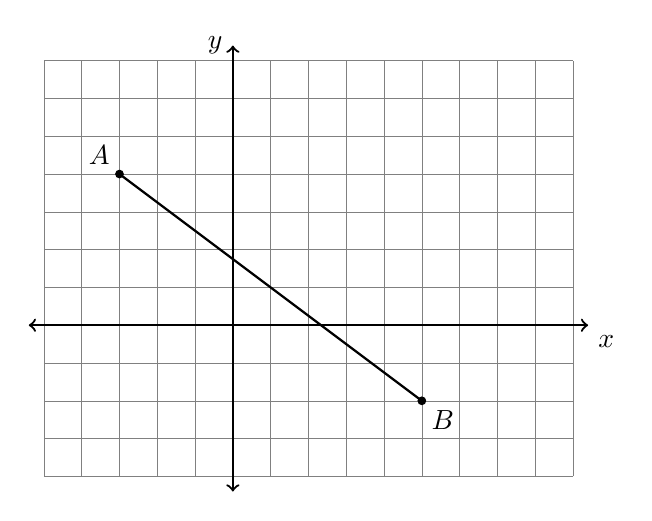
\begin{tikzpicture}[scale=.48]
        \draw [help lines] (-5,-4) grid (9,7);
        \draw [thick, <->] (-5.4,0) -- (9.4,0) node [below right] {$x$};
        \draw [thick, <->] (0,-4.4)--(0,7.4) node [left] {$y$};
        \draw [thick] (-3,4)--(5, -2);
        \draw [fill] (-3,4) circle [radius=0.1] node[above left] {$A$};
        \draw [fill] (5, -2) circle [radius=0.1] node[below right] {$B$};
      \end{tikzpicture}
    \end{flushright}

\item In the diagram below, $\overline{AC}$ has endpoints with coordinates $A(-3,-2)$ and $C(7, 3)$.\\[0.25cm]
  If $B$ is a point on $\overline{AC}$ and $AB {:} BC = 3{:}2$,  what  are  the coordinates of $B$?
    \begin{flushright} %4 quadrant regents grid
      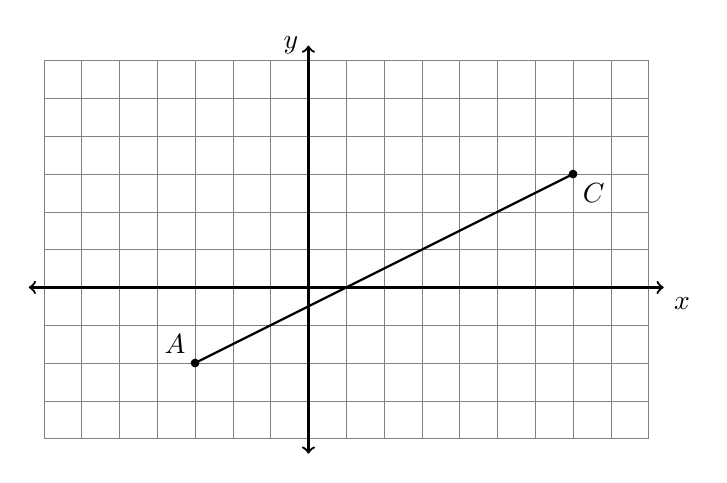
\begin{tikzpicture}[scale=.48]
        \draw [help lines] (-7,-4) grid (9,6);
        \draw [thick, <->] (-7.4,0) -- (9.4,0) node [below right] {$x$};
        \draw [thick, <->] (0,-4.4)--(0,6.4) node [left] {$y$};
        \draw [thick] (-3,-2)--(7, 3);
        \draw [fill] (-3,-2) circle [radius=0.1] node[above left] {$A$};
        \draw [fill] (7, 3) circle [radius=0.1] node[below right] {$C$};
      \end{tikzpicture}
    \end{flushright}

\newpage
\item Given $P(-2,7)$ and $Q(3,-5)$, find the length of $\overline{PQ}$.
      \vspace{4cm}

\item A translation maps $A(-1,14) \rightarrow A'(-11,4)$. What is the image of $B(1,-3)$ under the same translation?  \vspace{3cm}

\item On the graph, draw polygon ABCDEF with vertices A(1, 1), B(1, 4), C(3, 4), D(3, 7), E(8, 7), and F(8, 1). Find the perimeter and the area of the polygon.\\[1cm]
  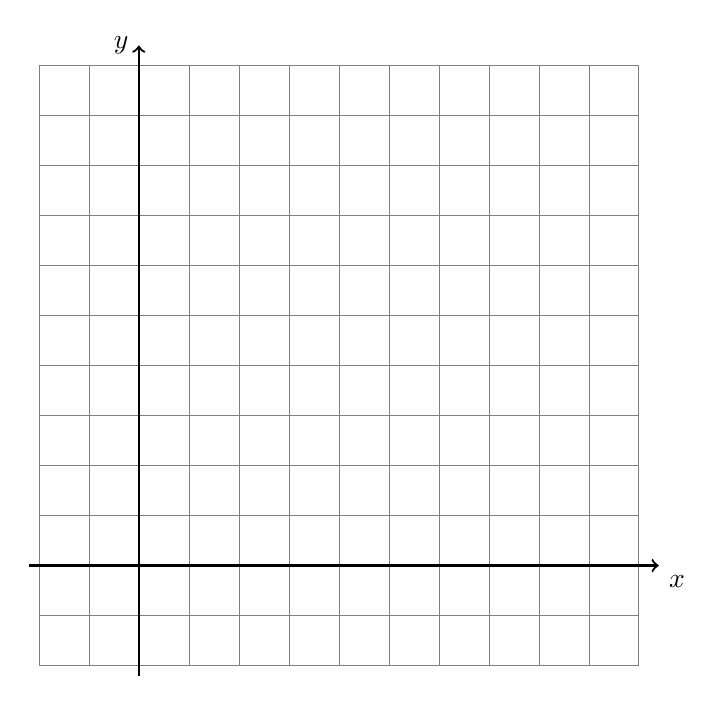
\begin{tikzpicture}[scale=.635]
    \draw [help lines] (-2,-2) grid (10,10);
    \draw [thick, ->] (-2.2,0) -- (10.4,0) node [below right] {$x$};
    \draw [thick, ->] (0,-2.2)--(0,10.4) node [left] {$y$};
  \end{tikzpicture}
  \vspace{2cm}

\newpage
\item Find the decimal value of each expression, rounded to the nearest hundredth.
  \begin{enumerate}
    \begin{multicols}{2}
    \item   $3 \sqrt{13}$ \vspace{1cm}
    \item   $\displaystyle \frac{3^2}{7}$
    \item   $1-\sqrt{5}$ \vspace{1cm}
    \item   $\displaystyle \frac{\pi}{4}$
    \end{multicols}
  \end{enumerate}
  \vspace{0.5cm}

\item In the following two problems, solve for the value of $x$.
    \begin{enumerate}
      \begin{multicols}{2}
      \item   $\frac{1}{5}(10x+5)=3$ \vspace{4cm}
      \item   $\frac{2}{3}(5-x)=-4$ \vspace{4cm}
      \end{multicols}
    \end{enumerate}
    \vspace{4cm}

\item Given $f(x)=\frac{1}{3} x+3$. Solve for $x$ such that for $f(x)=2$. \vspace{5cm}
\item Given $g(x)=-2x^2-5x+3$. Simplify $g(1)$. \vspace{2cm}

\newpage
\item Given $h(x)=x^2-4x-5$. Solve $h(x)=0$. \vspace{5cm}

\item Spicy: On the set of axes below, graph the quadrilateral $ABCD$ having coordinates $A(-2,-1)$, $B(5,1)$, $C(5,6)$, and $D(-2,4)$. \\*[0.25cm]
  Find the slope of each of the four sides. What type of quadrilateral is $ABCD$? Justify your answer.
  \begin{flushright} %4 quadrant regents grid
    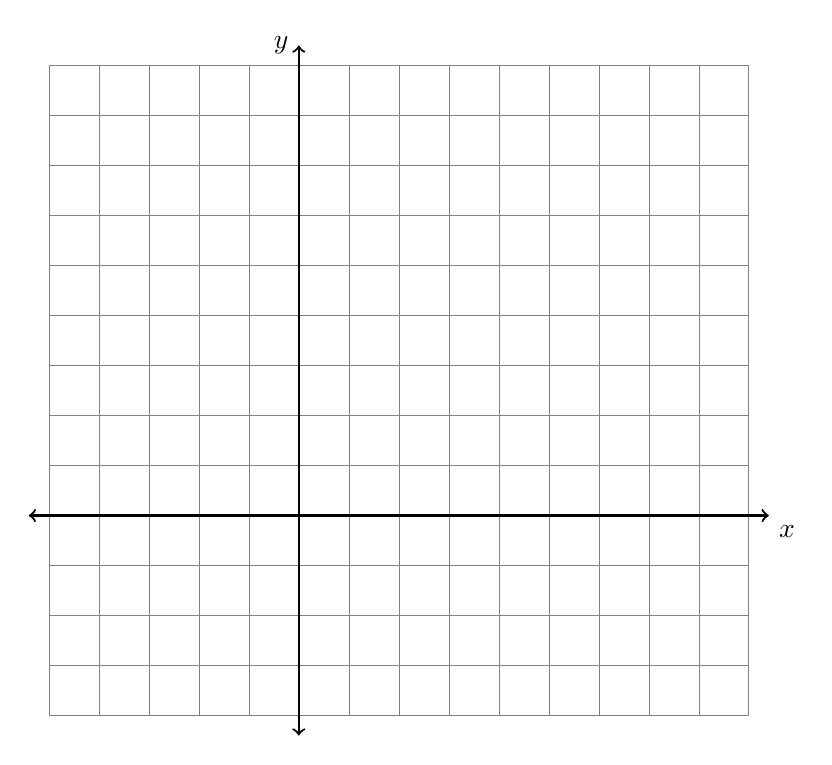
\begin{tikzpicture}[scale=.635]
      \draw [help lines] (-5,-4) grid (9,9);
      \draw [thick, <->] (-5.4,0) -- (9.4,0) node [below right] {$x$};
      \draw [thick, <->] (0,-4.4)--(0,9.4) node [left] {$y$};
      %\draw [thick] (-2,-1) node[below] {$A$}--
      %(5,1) node[right] {$B$}--
      %(5,6) node[right] {$C$}--
      %(-2,4) node[left] {$D$}--cycle;
    \end{tikzpicture}
  \end{flushright}

\end{enumerate}
\end{document}